
\documentclass[titlepage]{article}
\usepackage{graphicx} % Required for inserting images


\usepackage{titlesec}
\usepackage{placeins}
\usepackage{afterpage}
\usepackage{hyperref}
\usepackage[margin=1.0in]{geometry}

\title{ECS171 Group 8 Report}
\author{Boquan Fang, Rutvik Deo, Ishita Dutta, Zhuo Chen}
\date{June 2023}


\begin{document}

\begin{titlepage}
    \begin{center}
        \vspace*{6cm}

        \Huge
        \textbf{Playlist Fit Checking}

        \vspace{0.5cm}

        \LARGE
        \textbf{ECS171 Machine Learning}

        \textbf{Group 8 Project Report}

        \vspace{0.5cm}

        \Large
        \textbf{Group Members:}

        Boquan Fang, Rutvik Deo, Ishita Dutta, Zhuo Chen

        \vspace{0.5cm}

        \textbf{Github Repository:}

        \url{https://github.com/BoquanFang/ECS171_Term_Project.git}

        \vspace*{\fill}
    \end{center}
\end{titlepage}

% \maketitle



\section{Introduction}
Listening to music is a popular activity that people all over the world engage in. 
Everyone has their own music taste and their own way of listening to music.
Some people exclusively listen to music by picking a single album by a single artist 
and listening to it from beginning to end, but others curate playlists of music from
various albums by various artists. These playlists are often designed to suit specific
moods, feelings, or languages and it is important to the listening experience that the contents of
each playlist are consistent to avoid jarring the listener or inducing whiplash.

Prior to the creation of intelligent recommender systems such as those employed by 
Spotify and YouTube Music, humans would create playlists for themselves or for others
and thus would select songs for each playlist that both fit that playlist's desired mood
and are tonally similar to the other songs on the playlist. However, as such 
online music platforms emerged, they became ways of exploring new types of music cheaply.
Users did not have to spend money on physical media or digital rights to a song that they
might not enjoy, so they could listen to lots of music themselves to determine if they liked it
or not. Later, as content recommendation algorithms became stronger and amassed more data
to train on, automatic recommendation methods became a viable way for users of these platforms
to find new music to listen to without having to listen to all the songs themselves. 

Thus, the goal of this research paper is about determining whether a chosen song is similar enough to others in a given playlist to be accepted into that playlist based on the energy measure of the song. As defined by Spotify, the energy of a song is a measure of the perceptual intensity or activity of a song, and for our goal, the best variable on the way users sort their playlists by ear. This can be used for a listener who does not have the time to listen to every song more than once to choose what is a good song to add to their playlist; users are more likely
to enjoy songs that can fit into their existing playlists, especially those they listen to most.
Additionally, it can be used to generate entirely new playlists for users, starting from a small
playlist of a few of their favorite songs, and then repeatedly searching for and adding songs that
fit the energy of the newly-generated playlist. This creates completely new full-sized playlists 
with consistent energy and tone and potentially new songs that the user has not listened to before.
This will create a novel but still enjoyable listening experience. 

% TODO: cite this better
% https://www.diva-portal.org/smash/get/diva2:850112/FULLTEXT01.pdf
\section{Literature Review}
Some studies have been done on Spotify data. For example, Nijkamp et al. used the Spotify API
to investigate whether a song's popularity could be predicted based on its other features and found
that it could not. Pareek et al. also found that a random forest model could classify songs
as popular or unpopular with an accuracy of 86\%. Code AI managed to predict popularity with a KNN
model with an error of only 0.03\%. However, all of these studies are addressing the problem
of predicting popularity; there is currently a gap in knowledge surrounding the problem of fitting
songs into playlists.

One instance of using machine learning to recommend songs rather than predict their popularity is
Alexander Bricken's Gaussian Mixture model which recommend songs based on their Spotify API
features. Though this is not exactly the same as determining whether a song fits into a playlist,
it is similar and a useful starting point. Additionally, Aalto et al. examined the problem of 
playlist construction using PCA and approximate nearest-neighbors and found that their model 
outperformed human curators in qualitative testing.

\section{Dataset Description and Exploratory Analysis}
This project’s dataset is retrieved by the user-level interface from the Spotify developer API. With two given URLs to a playlist and a song, the user-level interface could access the Spotify developer API and save the data for both the playlist and the given song in a CSV file. The number of rows is depended on how many songs a given playlist has. The Spotify developer API provides thirteen attributes for a given song: name, danceability, energy, key, loudness, mode, speechiness, acousticness, instrumentalness, liveness, valence, tempo, and duration. The name represents the name of a given song and that would not be considered in our exploratory data analysis part. Danceability “describes how suitable a track is for dancing based on a combination of musical elements including tempo, rhythm stability, beat strength, and overall regularity.” Energy represents “a measure from 0.0 to 1.0 and represents a perceptual measure of intensity and activity.” The key represents the track that a given music is in. Loudness shows the overall loudness of a song in decibels.  Mode indicates “the modality (major or minor) of a track, the type of scale from which its melodic content is derived”. Speechiness indicates the presence of oral spoken words in the given song. Acousticness is the confidence interval of the track in terms of acoustic. Instrumentalness “predicts whether a track contains no vocals.” Liveness detects “the presence of an audience in the recording.” Valence is “a measure from 0.0 to 1.0 describing the musical positiveness conveyed by a track.” Temp covers “the overall estimated tempo of a track in beats per minute (BPM).” The attributes duration indicates the duration of the songs in millisecond. 


\section{Proposed Methodology}
To go about determining whether a song would match the energy of a playlist, we decided to do the following steps:
\begin{enumerate}
    \item Run the Spotify API to get the information for the input playlist and the test song.
    \item Preprocess our training set, or the given dataset of our playlist so that we were able to get a more standard method of measurement.
    \item Run the model and determine an energy category prediction for the new playlist
    \item Determine a conclusion based on the standard determination of the songs in the playlist.
\end{enumerate} 

To complete the first step, we visited the Spotify for Developers website [1]. In this, we were able to create a login key that would allow us to run the API for gathering song data. Here, we decided to parse the URL for the specific guid that would identify the public playlist. After a few more parameters, we were able to get our data and display it on our interface, as well as save the data to a file called \textbf{songs.csv}. We also did the same for the new song and saved that to a file called \textbf{rand\_song.csv}.
\\\\
From here, we started focusing on the model and specifications necessary for running the model properly. To do this while we were still figuring out the API, we decided to use a practice dataset from Kaggle [2]. Using this set covering the same variables over 20.0k songs, we learned more about the measures and what preprocessing steps we should take in order to have a standard model.For preprocessing our data, we decided to place all of our energy levels into a category called $`energy\_categories`$. What this did was create the buckets for the classification algorithms to predict the new song's energy level. To do this, we took the original energy between the interval  $[0.0, 1.0]$ and floor divided by 0.01 to have a maximum of 100 energy categories. We chose 0.01 for the most accuracy while still keeping the differences of the dataset and to make all the numbers integers (avoiding 0.5 values) to better classify into buckets. This helped create a more feasible output for the model, while still keeping the values as accurate as possible. We then made a histogram showing the distribution of the $`energy\_category`$ values. Here, we realized that, due to the law of large numbers, we would not need to worry too much about the normality of the data and carried on with the data normality assumption. This was due to observing not only the Kaggle dataset, but multiple playlists pulled from the spotify interface, all showing similar to bell curve histograms. We then dropped the $`Name`$ variable for having a more blind analysis, so that the model would not confuse the $`Name`$ as one of the evaluatory measures and skew the ouptut. From here, we decided to 
create the correlation heatmap of our data, so that we could determine the necessary variables for a more accurate analysis. We decided to do this for two endpoint reasons. The first reason was that we did not want to include all of the variables in our analysis. Some of the variables like `Mode` and $`Instrumentalness`$ were displaying really low correlations to the energy with our Kaggle dataset. Including these variables meant that we were introducing more noise to our model rather than giving it data to make a more accurate analysis. The second was to determine a sort of pattern that would tell us how to determine which variables were best for our model. To elaborate, we found that some variables correlate more than others when the playlist would change. Because of the lack of a static training set, we had to set preprocessing patterns such that we would be able to handle any given playlist. This meant that we would use a threshold for the correlation to the original $`Energy`$ variable so that we would be able to accommodate for all different correlation patterns. We chose the threshold 0.2 because we saw that for most data, we would have more than 2 variables for our X when we would have the threshold, so that became our sweet spot. A higher threshold meant we were not getting the necessary amount of variables for an accurate prediction, while the lower threshold meant having too much noise. After removing the unnecessary variables using a more dynamic code, we decided to plot the heatmap again to check that all the necessary variables were still in the dataset, and display which variables are being used. From there we ran our model.
\\\\
We chose two proposed methodologies when working on determining our conclusion. 
\\
One of the methodologies was running a polynomial regression model on our data.
The polynomial regression model is a model that follows a regression sense, in which each variable is assigned a constant to be multiplied to, so following the:
\\
The other method proposed was running a KNN model [3]. As described more in the source, this model is essentially classifying a new point based on the information from the training set for a certain number of neighbors. If this means that the number of neighbors is from category A, then the model will classify A, whereas if the neighbors are category B, then classify category B. This is classified using the Euclidian distance of the points as a vector(ie. each of the songs is a separate vector of all the x variables) For this model, we decided to keep our model as dynamic as possible and started looking at ways we could determine the k number of neighbors needed for the model. We decided on an $sqrt(n)$ [3] neighbor. Essentially, this means if we have 100 songs in our playlist, the model looks at the 10 nearest neighbors (but if the playlist number is something like 90 or a number between 2 perfect squares, it will round using the 0.5 rule). When running this model on the Kaggle dataset, we were able to achieve an average of 87\% accuracy when predicting 5 different song energy categories over multiple tests. 

\section{Experimental Results}
Comparing the results of the two models, we found that the KNN model was more consistent and accurate, so we decided to build our conclusions from the KNN model. In order to build our conclusion, we decided to compare the playlist energy mean to the classified prediction. In this, we took the mean and standard deviation of the $energy\_categories$ of the playlist before making them factor buckets. At the end of the model, we took the result and ran a Z-test [4] of the prediction to the mean of the playlist (this was done with the same normality assumption for the histogram) and plotted the results in Figure 5. The green lines indicated the 90\% confidence interval boundaries. The positioning of the red line would give us the conclusion for that song in relation to the given playlist. What this meant was that if the red line was inside the green lines, it was similar in energy to 90\% of the song data, else it was in the outlying 10\% of the energy of the songs in the playlist. We would determine the songs outside of the lines as "not a good fit" for the playlist, as we would have to be more careful about the placement of these songs in the playlist in relation to other songs. Songs within the green lines were "a good fit" for the playlist because there was a lower worry about the location placement of that song in the playlist in relation to other songs in the playlist.

\section{Interface Design}
\subsection{Interface Introduction}
Once we have developed the model, we should use Flask to create an API that allows users to input a playlist and get the desired results. Flask is a popular Python web framework that is suitable for building lightweight web applications and APIs.

\subsection{User Interface}
To create a website using Flask that allows users to input a playlist URL and extract its attributes, you'll need to perform the following steps:

1. Get an access token for the Spotify Web API:
You should first Register a new application on the Spotify Developer Dashboard (https://developer.spotify.com/dashboard/applications).
Obtain the client ID and client secret and then get the access token.\\
2. Use the access token to get the playlist data.\\
3. Get the song names and audio features from the playlist data\\
4. Creating a text box for a user to enter a single song's URL and retrieve its data.\\
5. Run the model on the page that we open, and get all the results based on our training model(the training dataset is the whole playlist, and the test dataset is the song that we enter.


\subsection{API: Get the song names and audio features from the playlist data}
You should first make a get request to the API URL. Then, parse the response to retrieve the relevant information. The response will include an array of track objects, each containing various details about the track. To accomplish the tasks mentioned, we need to create four HTML files: \textbf{index.html, music.html, song.html,} and \begin{itemize} 
    \item \textbf{index.html}: This file will serve as the welcome
        page where users can enter the playlist URL. It should contain necessary
        HTML elements such as input fields, buttons, and a form to gather user
        input.  
    \item \textbf{music.html}: This file will include essential code for
        integrating with the Spotify API or any other music-related functionality
        you're implementing.  
    \item \textbf{songs.html}: This file is essential for
        displaying song attributes and allowing users to select a single song as a
        test case. It should include HTML elements to show song details such as
        title, artist, album, and other relevant information.  
    \item \textbf{song.html}: This file will display detailed information about a
        single song, including its attributes and several graphs to support your
        model. Additionally, it can include the final test result to assess the
        model's performance. It uses HTML elements like headings, paragraphs,
        charts, or visualizations to present the information effectively.
\end{itemize}
This is explained in order by the figures in section 8. Figure 1 captures the link to the playlist and starts gathering data. We then move to Figure 2, in which we display the information for all of our songs on the playlist for the user to verify the correct songs being pulled. We scroll down to Figure 3, in which we provide the Spotify link of the new song we are trying to test for. This makes our data dynamic, as our training and testing set are both provided by our user, making our model more streamlined to handle any kind of playlist regardless of mood, or language. Figure 4 starts displaying our results, which include the original heatmap of the data, then the remade heatmap of the dropped variables as well as the distribution of the histogram of the playlist song $energy\_category$ values. Scrolling down again, Figure 5 displays the normal curve of our Z test as well as our conclusion.


\section{Conclusion and Discussion}
Comparing the results of the two models, we found that the KNN model was more consistent and accurate, so we decided to build our conclusions from the KNN model. In order to build our conclusion, we decided to compare the playlist energy mean to the classified prediction. In this, we took the mean and standard deviation of the $energy\_categories$ of the playlist before making them factor buckets. At the end of the model, we took the result and ran a Z-test of the prediction to the mean of the playlist (this was done with the same normality assumption for the histogram) and plotted the results in Figure 5. The green lines indicated the 90\% confidence interval boundaries. The positioning of the red line would give us the conclusion for that song in relation to the given playlist. What this meant was that if the red line was inside the green lines, it was similar in energy to 90\% of the song data, else it was in the outlying 10\% of the energy of the songs in the playlist. We would determine the songs outside of the lines as "not a good fit" for the playlist, as we would have to be more careful about the placement of these songs in the playlist in relation to other songs. Songs within the green lines were "a good fit" for the playlist because there was a lower worry about the location placement of that song in the playlist in relation to other songs in the playlist.                                                                                                                               The conclusions were drawn based on the KNN model's predictions, which were compared to the playlist's energy mean. The positioning of the red line in relation to the green lines determined whether a song was a good fit or not.

\section{Figures}
\begin{figure}[!h]
\centering
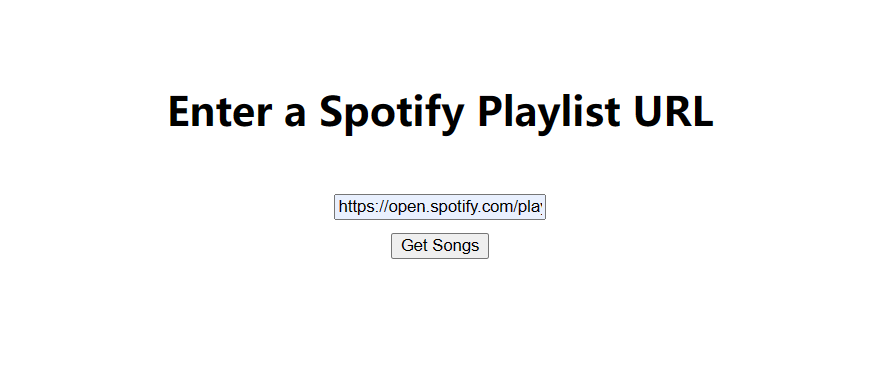
\includegraphics[width=1\textwidth]{1.png}
\caption{This is the welcome page of the user interface}
The user could enter any playlist URL here.
\label{fig:enter-label}
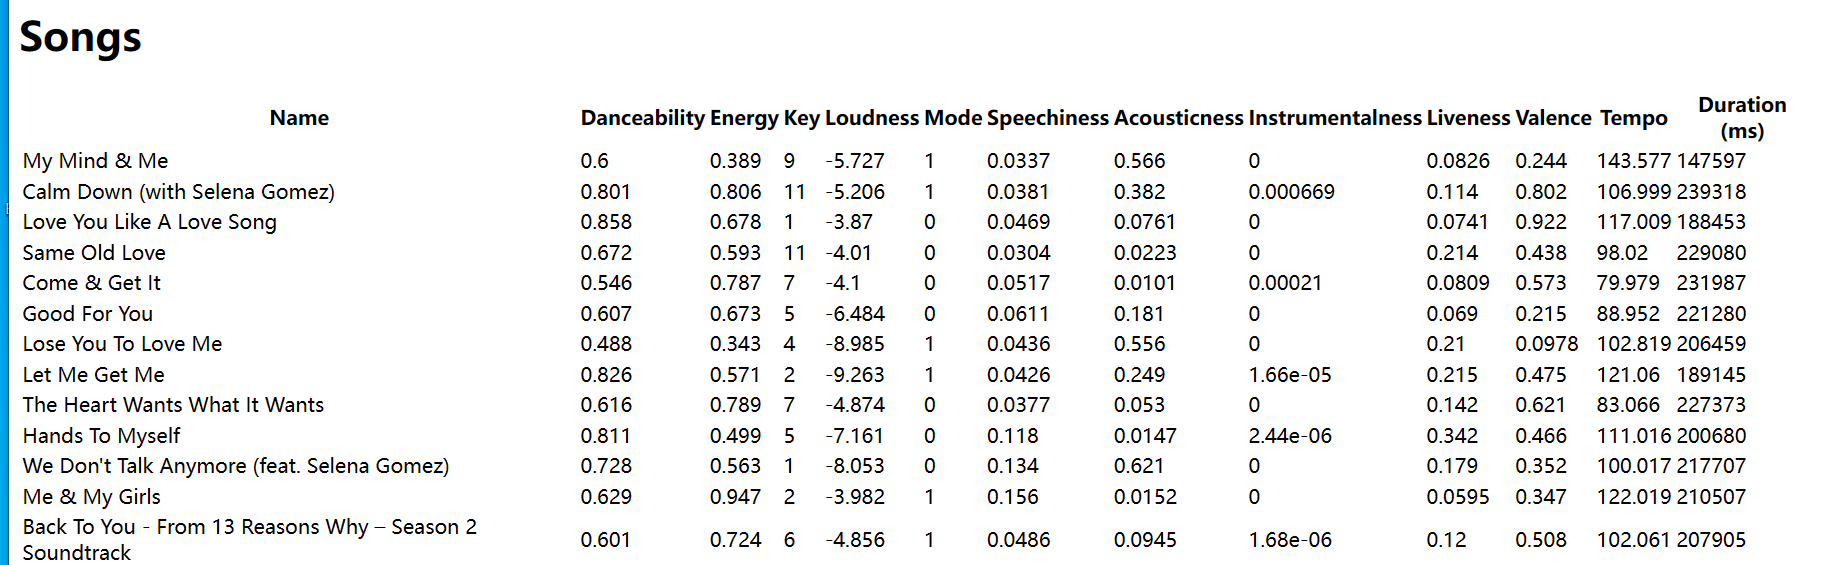
\includegraphics[width=1\textwidth]{2.png}
\caption{This is the attribute that we extract from the playlist.}

\includegraphics[width=0.5\textwidth]{3.png}
\caption{The user can enter any song's URL as the test dataset here.}
\end{figure}

\begin{figure}[h]
\centering
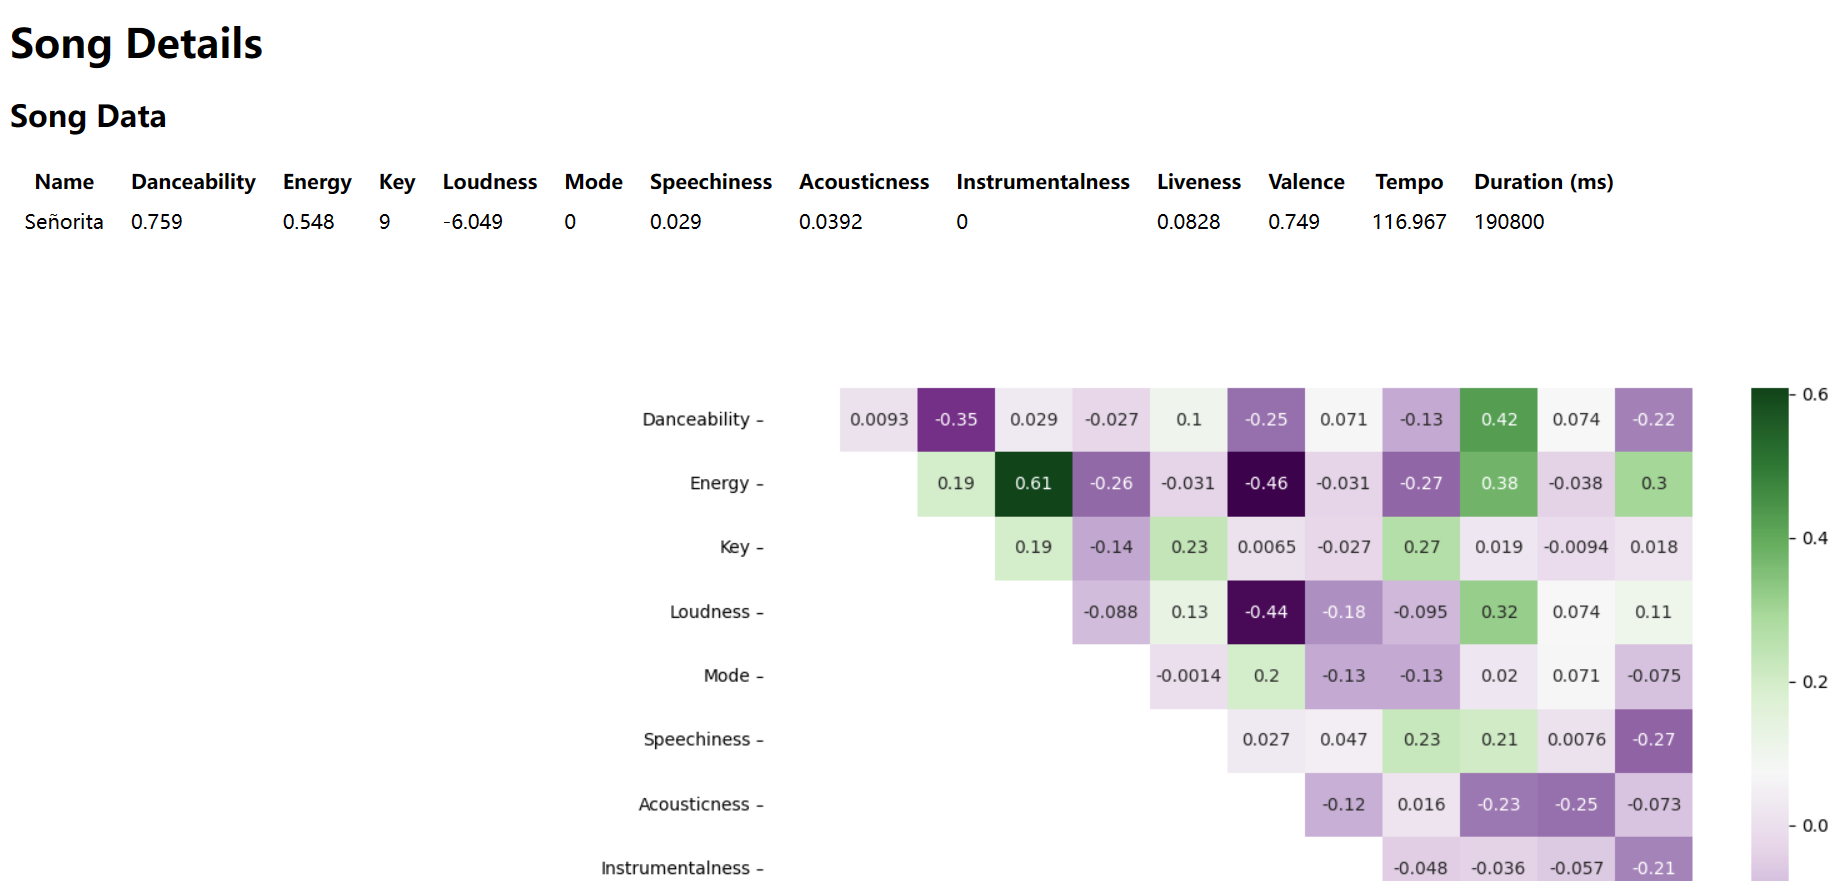
\includegraphics[width=1\textwidth]{4.png}
\caption{Here is a new page after the user enters the song's URL with the attributes of the song and the initial heatmap of the playlist}


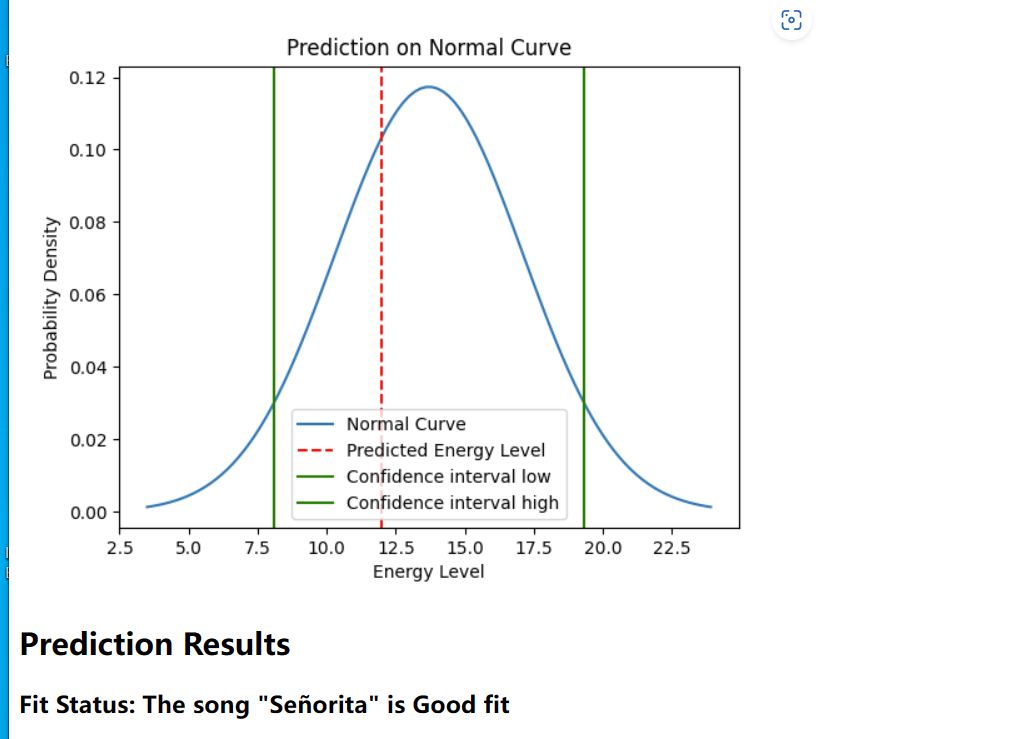
\includegraphics[width=1\textwidth]{5.png}
\caption{Finally, it shows the result at the bottom of the page about whether this song's style is similar to our playlist.}
\label{fig:enter-label}
\end{figure}

\clearpage
\section{Sources Cited}
\begin{enumerate}
    \item
    Analytics Vidhya. "Traversing the Trinity of Statistical Inference – Part 2: Confidence Intervals." Analytics Vidhya, Analytics Vidhya Pvt. Ltd., 15 June 2021, https://www.analyticsvidhya.com/blog/2021/06/traversing-the-trinity-of-statistical-inference-part-2-confidence-intervals/.
    \item
    Chattopadhyay, Manojit. "How to Find the Optimal Value of K in KNN." Towards Data Science, Towards Data Science, 7 Nov. 2019, https://towardsdatascience.com/how-to-find-the-optimal-value-of-k-in-knn-35d936e554eb.
    \item 
    Noor, Muhammad. "Statistical Inference in Big Data Era." DiVA Portal, Uppsala University, 2015, https://www.diva-portal.org/smash/get/diva2:850112/FULLTEXT01.pdf.
    \item 
    Rastelli, Salvatore. "Spotify and YouTube." Kaggle, Kaggle, n.d., https://www.kaggle.com/datasets/salvatorerastelli/spotify-and-youtube.
    \item 
    Spotify. "Web API." Spotify for Developers, Spotify AB, n.d., https://developer.spotify.com/documentation/web-api.
\end{enumerate}
\end{document}
